% This is "sig-alternate.tex" V2.0 May 2012
% This file should be compiled with V2.5 of "sig-alternate.cls" May 2012
%
% This example file demonstrates the use of the 'sig-alternate.cls'
% V2.5 LaTeX2e document class file. It is for those submitting
% articles to ACM Conference Proceedings WHO DO NOT WISH TO
% STRICTLY ADHERE TO THE SIGS (PUBS-BOARD-ENDORSED) STYLE.
% The 'sig-alternate.cls' file will produce a similar-looking,
% albeit, 'tighter' paper resulting in, invariably, fewer pages.
%
% ----------------------------------------------------------------------------------------------------------------
% This .tex file (and associated .cls V2.5) produces:
%       1) The Permission Statement
%       2) The Conference (location) Info information
%       3) The Copyright Line with ACM data
%       4) NO page numbers
%
% as against the acm_proc_article-sp.cls file which
% DOES NOT produce 1) thru' 3) above.
%
% Using 'sig-alternate.cls' you have control, however, from within
% the source .tex file, over both the CopyrightYear
% (defaulted to 200X) and the ACM Copyright Data
% (defaulted to X-XXXXX-XX-X/XX/XX).
% e.g.
% \CopyrightYear{2007} will cause 2007 to appear in the copyright line.
% \crdata{0-12345-67-8/90/12} will cause 0-12345-67-8/90/12 to appear in the copyright line.
%
% ---------------------------------------------------------------------------------------------------------------
% This .tex source is an example which *does* use
% the .bib file (from which the .bbl file % is produced).
% REMEMBER HOWEVER: After having produced the .bbl file,
% and prior to final submission, you *NEED* to 'insert'
% your .bbl file into your source .tex file so as to provide
% ONE 'self-contained' source file.
%
% ================= IF YOU HAVE QUESTIONS =======================
% Questions regarding the SIGS styles, SIGS policies and
% procedures, Conferences etc. should be sent to
% Adrienne Griscti (griscti@acm.org)
%
% Technical questions _only_ to
% Gerald Murray (murray@hq.acm.org)
% ===============================================================
%
% For tracking purposes - this is V2.0 - May 2012

\documentclass{sig-alternate}
\usepackage{epstopdf}
\usepackage{algorithm2e}
\usepackage{multirow}
\usepackage{hyperref}
%\usepackage{auto-pst-pdf}
\begin{document}
%
% --- Author Metadata here ---
\conferenceinfo{GECCO2014}{2014 Victoria, BC, Canada}
%\CopyrightYear{2007} % Allows default copyright year (20XX) to be over-ridden - IF NEED BE.
%\crdata{0-12345-67-8/90/01}  % Allows default copyright data (0-89791-88-6/97/05) to be over-ridden - IF NEED BE.
% --- End of Author Metadata ---

\title{Enhancing the Performance of Genetic Algorithms in Combinatorial Optimization of Large and Difficult Problems}
\subtitle{Using Variable Adaptive Mutation Rates Controlled by 'Inbreeding'}
%
% You need the command \numberofauthors to handle the 'placement
% and alignment' of the authors beneath the title.
%
% For aesthetic reasons, we recommend 'three authors at a time'
% i.e. three 'name/affiliation blocks' be placed beneath the title.
%
% NOTE: You are NOT restricted in how many 'rows' of
% "name/affiliations" may appear. We just ask that you restrict
% the number of 'columns' to three.
%
% Because of the available 'opening page real-estate'
% we ask you to refrain from putting more than six authors
% (two rows with three columns) beneath the article title.
% More than six makes the first-page appear very cluttered indeed.
%
% Use the \alignauthor commands to handle the names
% and affiliations for an 'aesthetic maximum' of six authors.
% Add names, affiliations, addresses for
% the seventh etc. author(s) as the argument for the
% \additionalauthors command.
% These 'additional authors' will be output/set for you
% without further effort on your part as the last section in
% the body of your article BEFORE References or any Appendices.

\numberofauthors{4} %  in this sample file, there are a *total*
% of EIGHT authors. SIX appear on the 'first-page' (for formatting
% reasons) and the remaining two appear in the \additionalauthors section.
%
\author{
% You can go ahead and credit any number of authors here,
% e.g. one 'row of three' or two rows (consisting of one row of three
% and a second row of one, two or three).
%
% The command \alignauthor (no curly braces needed) should
% precede each author name, affiliation/snail-mail address and
% e-mail address. Additionally, tag each line of
% affiliation/address with \affaddr, and tag the
% e-mail address with \email.
%
% 1st. author
\alignauthor
Daniel Smullen\titlenote{Corresponding author.}\\
       \affaddr{UOIT}\\
       \affaddr{2000 Simcoe St. N}\\
       \affaddr{Oshawa, ON, Canada}\\
       \email{daniel.smullen@uoit.net}
% 2nd. author
\alignauthor
Jonathan Gillett\\
       \affaddr{UOIT}\\
       \affaddr{2000 Simcoe St. N}\\
       \affaddr{Oshawa, ON, Canada}\\
       \email{jonathan.gillett@uoit.net}
% 3rd. author
\alignauthor
Joseph Heron\\
       \affaddr{UOIT}\\
       \affaddr{2000 Simcoe St. N}\\
       \affaddr{Oshawa, ON, Canada}\\
       \email{joseph.heron@uoit.net}
\and  % use '\and' if you need 'another row' of author names
% 4th. author
\alignauthor Shahryar Rahnamayan\\
       \affaddr{UOIT}\\
       \affaddr{2000 Simcoe St. N}\\
       \affaddr{Oshawa, ON, Canada}\\
       \email{shahryar.rahnamayan@uoit.ca}
}
% There's nothing stopping you putting the seventh, eighth, etc.
% author on the opening page (as the 'third row') but we ask,
% for aesthetic reasons that you place these 'additional authors'
% in the \additional authors block, viz.
\additionalauthors{}
% Just remember to make sure that the TOTAL number of authors
% is the number that will appear on the first page PLUS the
% number that will appear in the \additionalauthors section.

\maketitle
\begin{abstract}
Blah blah blah, here is our abstract.
\end{abstract}

\keywords{Genetic Algorithms, Combinatorial Optimization, N Queens Problem, Variable Mutation}




%%%%%%%%%%%%%%%%%%%%%%%%%%%%%%%%%%%%%%%%%%%%%%%%%%%%%%%%%%%%%%%%%
% 
% INTRODUCTION
%
%%%%%%%%%%%%%%%%%%%%%%%%%%%%%%%%%%%%%%%%%%%%%%%%%%%%%%%%%%%%%%%%%
\section{Introduction}
Genetic algorithms serve an important role in various applications, but particularly useful areas are those where they can perform stochastic generation of solutions for combinatorial problems. One notable example of this is the N-Queens problem. One approach to solving the N-Queens problem using a genetic algorithm is to implement chromosomes which model the position of each queen on the chessboard. The permuted values stored in the chromosome represent the sequential row positions of each queen, encoded into binary values. Each column value is the index, since there can never be more than one queen per column. Thus, the column positions increase by one for each queen and the intersections (referred to as collisions) are calculated per row or on the diagonal to determine whether a solution has been found. As with any genetic algorithm, evaluating the fitness of the chromosomes per generation is required to determine if a usable solution has been generated. 

By tuning the parameters of the genetic algorithm, performance can increase or decrease based on the solution landscape of the problem encountered. We have found that by replacing a static mutation value with an adaptive value controlled by chromosome similarity, better performance can be achieved than using static values, particularly when there is no \emph{a priori} knowledge about the ideal static mutation rate. This is compounded when the solution landscape is large, such as in higher-order N-Queens problems.

\subsection{Background and Problem Domain}
Like many other complex optimization problems, the N-Queens problem becomes orders of magnitude more complex as the number of queens and the size of the chessboard increases. Finding all solutions is a simple but non-trivial problem. When two or more queens share a row or diagonal, a collision occurs for each pair of queens, meaning that the board state is not a solution.

The Eight-Queens problem is the classical version of the puzzle, and even with this configuration the problem is computationally expensive. There are {$64 \choose 8$} arrangements of the queens on a standard {$8\times{}8$} board. Exhaustive deterministic evaluation has shown that there are only 92 distinct solutions. Even including optimizations such as imposing a constraint to place only one queen to a single row, there are still {$8^8$} possible distinct arrangements. In higher-order versions of the problem, combinatorial explosion occurs. The Nine-Queens problem has 352 distinct solutions. The Ten-Queens problem has 724. Table \ref{table:numuniquesol} in section \ref{tablesection} shows the growth of the number of solutions. 

While the number of solutions is known for problems involving up to 26 queens, there is currently no known formula to determine the exact number of distinct solutions. That is to say, higher order N-Queens problems are currently intractable with existing methods. Deterministic methods for approaching these problems are largely useless, and the problem remains unsolved.

- (ADD CITATIONS!
  
% CITATIONS EXAMPLE WITH ALL CITATATIONS
- Cite me!\cite{crawford1992solving,homaifar1992e1,andrews2006investigation,tuson1998adapting, wolpert1997no,srinivas1994adaptive,goldberg1988genetic}

\subsubsection{The N-Queens Puzzle}
The natural question raised when approaching simple problems is why a deterministic or brute force strategy is not used. Unfortunately, these approaches cannot work within human time-frames except in smaller problem landscapes. The issue is that a direct linear traversal of the landscape does not yield fruitful results easily in the case of the N-Queens problem. This stems from the fact that the fitness of each sequential solution doesn't matter. The problem cannot be solved by producing a solution that has queens which will attack each other. Therefore, only solutions with the absolute maximum, 100\% fitness, are useful solutions. What is more, as the problem landscape increases in size, the number of distinct solutions does not increase proportionally. A full brute force traversal of the landscape would be required to find all the distinct solutions, which is increasingly expensive in higher order problems.

Other stochastic solutions are impractical with this type of problem. This is because finding solutions among the landscape of possible board states yields a tremendous amount of duplicate solutions. Some method is required to direct the random traversal of the landscape toward distinct solutions and away from those which have already been found. The problem with this statement, is that the nature of randomness cannot be constrained in this way - it will no longer be random. Therefore methods such as genetic algorithms become an attractive solution approach  because they represent a 'smarter' traversal of the problem landscape than what is offered by a linear brute force traversal, or a uniformly random traversal of the landscape. Less time is spent on areas of the landscape which are not likely to be solutions. This leads us toward the core motivation of our solution's behavior.

- (ADD CITATIONS!)

\subsubsection{Motivation}\label{motivation_section}
Modeling the randomness of the solution landscape as seen in the N-Queens problem is impossible with known mathematical methods. To produce a geometric solution landscape would require that the dependent axis of the coordinate plane maps each sequential value to a uniformly random value in the actual solution landscape. Conceptually this is very difficult to imagine, but the reason why this conceptual strategy is useful will become clearer. First, we will discuss why a new approach is necessary in comparison to traditional GA approaches.

There are several 'short-cuts' which are available when approaching the N-Queens problem because of the nature of the chess board. Since it is square, one solution in fact can be used to yield many other unique solutions using symmetry operations (reflection and rotation of the board). This means that up to 8 solutions can be generated by finding one distinct solution. However, symmetry operations cannot be used to find all distinct solutions because many symmetrical configurations of the board are equivalent. In the example of the Eight-Queens problem, there are 11 board configurations which yield 8 solutions, and 1 which yields only 4. The result is still 92 unique solutions, with the majority of them calculable through symmetry operations alone.

Using symmetry operations, our initial exploration into solving the N-Queens problem yielded solutions quickly, but not quickly enough to beat deterministic solution generation methods. This was especially apparent in lower order problems where the solution landscape is small. We began to explore biological definitions of genetics, and sought inspiration from the fact that nature has an apparent system for maintaining genetic variation within organisms. For example pure-bred dogs often tend to have significant health problems which directly result from inbreeding. Royal families historically used inbreeding to keep their line 'pure', which also resulted in genetic abnormalities. (CITE THIS)

These facts led us toward a theoretical approach to apply the negative effects of inbreeding towards genetic algorithms. Our approach would make the mutation rate variable based on chromosome similarity, suggesting the natural mutant products of inbreeding as a result of a too-similar biological chromosome. Our initial solution worked exceptionally well, providing all 92 solutions nearly instantaneously in comparison to our previous static mutation rate GA which required a few seconds. This motivated us to pursue the implications of our strategy further.

\subsection{Related Work}

- This is where you can cite all of the references Joseph found regarding other types of variable mutation.
- Joseph DO THIS




%%%%%%%%%%%%%%%%%%%%%%%%%%%%%%%%%%%%%%%%%%%%%%%%%%%%%%%%%%%%%%%%%
% 
% APPROACH
%
%%%%%%%%%%%%%%%%%%%%%%%%%%%%%%%%%%%%%%%%%%%%%%%%%%%%%%%%%%%%%%%%%
\section{Our Solution Approach}
Ordinary genetic algorithms use three parameters to govern their evaluation. The first is the population size. We have not adjusted this parameter in our experiments, and kept them at a fixed value of 64 chromosomes. Second is the chromosome crossover rate, which governs the likelihood and percentage of a chromosome to splice with another. This was also kept static, at a fixed rate of 70\%. The third parameter is mutation rate, which governs the likelihood that a chromosome will have a random gene modified. This is achieved using a bit-flipping operation on the selected gene's binary encoded values. To support the 'in-breeding' variant of the algorithm, we have selected to replace the fixed mutation rate parameter with a variable rate, governed by a separate parameter which was kept at a fixed value for the sake of experimentation. The separate parameter, chromosome similarity threshold, is expressed as a percentage. We have selected 15\% as an arbitrary threshold which seemed to work well during experimentation. Future studies into the nature of this parameter may yet yield improved results for specific circumstances. The offset by which the mutation rate is adjusted (based on the chromosome similarity parameter) is set at a fixed value of 1\%.

(cite paper justifying why we used these values, they are often recommended/used values, Genetic Algorithms by Goldberg)


\subsection{Applying Adaptive Variable Mutation Rates}
In order to apply our adaptive variable mutation rate, a two step process is required. For each generation of chromosomes, the population chromosome similarity must be evaluated. The similarity algorithm is detailed in a separate subsection.  

When the chromosome similarity is less than the specified threshold, the mutation rate must decrease. For the next generation, the mutation rate is decreased. If the chromosome similarity increases again, and it goes above the specified threshold, the mutation rate decreases. Due to the stochastic nature of the algorithm, wild variations in chromosome similarity may result regardless of the mutation rate. Since the crossover of the genes may be up to 70\%, the resultant permutations of the genome are likely to be similar unless some mutation occurs. The result of this adaptive change in mutation rate is that the chromosome similarity will approach an equilibrium close to the specified inbreeding threshold.

% This is essentially explaining the chromosome similarity algroithm since the concept of 
% applying variable mutation from the previous subsection can be easily explained in words 
% without a formal algorithm.
\subsubsection{Chromosome Similarity Algorithm}
Chromosome similarity is calculated using a greedy algorithm seen in Algorithm \ref{alg:similarity}. First, the chromosomes' genes are decoded into integer values by direct translation of their binary values in sequence to an integer. next, the array of chromosomes' integer representations is sorted. Our implementation uses the quick-sort algorithm for minimal computational overhead. This gives the algorithm its' characteristic asymptotic behavior, as the complexity of the actual sorting function itself is of higher complexity than the main similarity calculation algorithm. That is to say, the sorting function used runs on average in $O(n \log n)$ complexity, although it should be noted that in the theoretical worst case, quick-sort works in $O(n^2)$ which is highly unlikely. The main algorithm runs in $O(n)$ linear complexity.

\begin{algorithm}
  \SetKwProg{Fn}{Function}{}{end}\SetKwFunction{Similarity}{Similarity}%
  \SetKwData{Similar}{similar}\SetKwData{Value}{value}\SetKwData{Matched}{matched}\SetKwData{Length}{length}\SetKwArray{Sorted}{sorted}
  \SetKwFunction{Sort}{Sort}
  \SetKwInOut{Input}{input}\SetKwInOut{Output}{output}
  \SetAlgoLined
  \DontPrintSemicolon
  
  \Fn{\Similarity{$chromosomes$}}{
  
  \Input{An array of $chromosomes$}
  \Output{Fraction of chromosomes that are similar}
  \BlankLine
  
  \Similar $\leftarrow$ 0\;
  \Matched $\leftarrow$ false\;
  \Length $\leftarrow$ length of $chromosomes$\;
  \BlankLine
  
  \tcp{Sort using an arbitrary sorting algorithm}
  \Sorted $\leftarrow$ \Sort{$chromosomes$}\;
  \BlankLine
  
  \For{$i \leftarrow 0$ \KwTo $\Length -1$}
  {
    \uIf{\Sorted{$i$} == \Sorted{$i + 1$}}
    {
      \Similar $\leftarrow$ \Similar + 1\;
      \Matched $\leftarrow$ true\;
    }
    \ElseIf{\Matched}
    {
      \Similar $\leftarrow$ \Similar + 1\;
      \Matched $\leftarrow$ false\;
    }
    \BlankLine
    
    \tcp{Case where the last item is a match}
    \If{\Matched and $\left(i + 1 == \Length - 1 \right)$}
    {
      \Similar $\leftarrow$ \Similar + 1\;
    }
  }
  \BlankLine
  \KwRet{\Similar / \Length}
  }
\caption{Chromosome similarity function}
\label{alg:similarity}
\end{algorithm}




% I thought it would be important to add a section on implementation
% this could be condensed, but I think it is very important to
% explain how we actually implemented and applied the GA process
\subsection{Implementation Specific Considerations}
In order to gain an appreciation for the specific implementation and how it might compare to alternatives, we will attempt to elaborate upon the special implementation considerations we made. Our experiments were performed on the same code as our development code, which was written in Java. Concurrent agile development was used as our main development methodology, and GitHub was used extensively for version management and simultaneous development of the code, documentation, and this report. 

The project source code is available at \url{http://www.github.com/gnu-user/}

% This is the design of the chromosome, which is important to the implementation details
\subsubsection{Chromosome Design}
Chromosomes are designed with an optimization that allow the stochastic search space to be minimized significantly, mentioned originally in section \ref{motivation_section}. The result is that the dimensionality of the problem decreases. This is accomplished by encoding each gene as a row (or column) position on the chess board, and each single index in the array of values means there can only be one queen placed at each index. This allows for an extendable chromosome up to N. Figure \ref{fig:chromosome} shows this chromosome pictorially for a $7 \times 7$ chessboard. In the figure, the 4th, 5th and 6th rows are not shown, but are filled with a queen at the 4th, 5th and 6th column positions respectively in this chromosome. As a result, the encoded chromosome is represented by 7 Java Integer class values in sequence. To encode this into one mutable array, the integers are simply concatenated together. The array specified in Figure \ref{fig:chromosome} would thus be translated to $1274563$.

\begin{figure}\label{fig:chromosome}
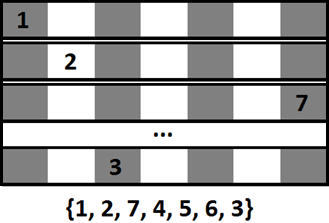
\includegraphics[width=0.5\textwidth]{chromosome.png}
\caption{Illustrating the chromosome data structure.}
\end{figure}

% The implementation detail of the fitness funciton including the algorithm
\subsubsection{Fitness Function}
Fitness is evaluated by determining the number of collisions between queens on the chessboard - in other words, when at least two queens can attack each other, a collision occurs for each queen. This means that in a board state where only one queen can attack another, two collisions result. Because it is impossible for there to be more than one queen per column given the data structure, only collisions across rows and diagonals must be found. The algorithm for determining the fitness of a given board state is given in Algorithm \ref{fitness_algorithm}, showing the mechanisms we used to find collisions across rows and diagonals. The fitness is calculated as $1 - \frac{1}{(1/N)}$, where the maximum fitness (a unique board solution) is $1$. The length of the chromosome corresponds to the number of queens and rows on the square chessboard, $N$.
 
\begin{algorithm}\label{fitness_algorithm}
  \SetKwProg{Fn}{Function}{}{end}\SetKwFunction{Fitness}{Fitness}%
  \SetKwData{Collisions}{collisions}\SetKwData{Length}{length}\SetKwArray{Chromosome}{$chromosome$}\SetKwData{Yi}{$y_i$}\SetKwData{Yj}{$y_j$}
  \SetKwFunction{Abs}{abs}
  \SetKwInOut{Input}{input}\SetKwInOut{Output}{output}
  \SetAlgoLined
  \DontPrintSemicolon
  
  \Fn{\Fitness{$chromosome$}}
  {
    \Input{A single $chromosome$}
    \Output{A fitness value for the chromosome}
    \BlankLine
    
    \Collisions $\leftarrow$ 0\;
    \Length $\leftarrow$ length of the $chromosome$\;
    \BlankLine
    
    \For{$i \leftarrow 0$ \KwTo $\Length -1$}
    {
      \tcp{Check each gene against the current}
      $j \leftarrow \left( i + 1 \right) \mod{\Length}$\;
      \While{$j$ != $i$}
      {
        \Yi $\leftarrow \Chromosome{i}$\;
        \Yj $\leftarrow \Chromosome{j}$\;
        \BlankLine
        
        \tcp{Check for vertical collision}
        \If{\Yi == \Yj}
        {
          \Collisions $\leftarrow \Collisions + 1$\; 
        }
        \BlankLine
        
        \tcp{Check for diagonal collision}
        \If{\Abs{$\left(i - j \right)$ / $\left(\Yi - \Yj \right)$} == 1}
        {
          \Collisions $\leftarrow \Collisions + 1$\;
        }
        \BlankLine
        
        $j \leftarrow j + 1$\;
        $j \leftarrow j \mod{\Length}$\;
      }
    }
    \BlankLine

    \eIf{\Collisions == 0}
    {
      \KwRet{1}\;
    }
    {
      \KwRet{1 / \Collisions}\;
    }
  }
\caption{Fitness function}
\label{alg:fitness}
\end{algorithm}

% The selection method, we use roulette wheel, however the implementation details of how
% roulette wheel is implemented is important
\subsubsection{Selection Method}
- Roulette wheel selection method, by generating a random floating point number and selecting
  a chromosome value where the random number lies within the bounds. The range
  of random values that can be chosen changes based on the maximum upper and lower
  bounds of the sum of the fitness of the chromosomes in the population.

- Each of the ranges of values that a particular chromosome can have is weighted
  based on the fitness of the chromosome. For example in a population with 4
  chromosomes two of which are solutions (fitness 1) and two with a single pair of collisions
  (fitness 1/2 = 0.5) the ranges of values for each chromosome would be as
  follows:

  [0, 1), [1, 2), [2, 2.5), [2.5, 3), and the bounds of the random floating point value
  generated for the roulette wheel selection would be [0, 3).


% The operations, these are pretty standard but we need to cite why we chose 70% and 30%
% we used these because they were recommended (e.g. from AI lectures) but need textbooks
% or papers to suggest why we used them
\subsubsection{Chromosome Operations}
- Crossover operation (70\% chance), cloning (30\% chance), 

- Background mutation operation, applied to chromosomes, this is variable rather
  than a traditional fixed value, e.g. a 5\% value results in a 5\% chance of
  mutation being applied to chromosomes.

- Mutation operator changes ONE of the genes of the chromosome randomly, which
  results in changing the the y coordinate of a random queen in the chromosome 
  to a random value within the range of possible y values.

- Mutation operator DOES NOT result in an invalid chromosome, it is limited to the
  range of possible (valid) y values.


% How we evaluate chromosomes in the population and determine distinct solutions
% and apply rotate and reflection to find additional solutions
% The use of terminology here is important DISTINCT implies that the particular
% arrangment of queens is different from another rotation/reflection of the same original
% solution. UNIQUE would consider all reflections/rotations as ONE "unique" solution
\subsubsection{Chromosome Evaluation}
- If a chromsome of the current population has a fitness value of 1 it is compared 
  to the list of previous solutions to see if it is unique. If the solution is 
  distinct the rotation (rotating the solution an additional three times) and 
  reflection (performing reflection on the solution) followed by three additional
  rotations operations are applied to find a total of 8 solutions. Each solution 
  found after rotation and reflection is compared to the list of previous solutions to 
  verify that it is a distinct solution.

  --> We do not keep duplicate solutions, this is important since someone may think
      that out of the 1000's of solutions we found many of them are just duplicates,
      when in fact they are all DISTINCT solutions.

- The current population is then replaced with the new population that was created
  by applying the crossover, cloning, and mutation operations.


% I would instead call this methodology and make testing/validation/etc. subsections
%\subsubsection{Testing and Validation}
\subsection{Experimental Methodology}

- Implementation in Java

- Experiments were conducted on the HPC facilities provided by SHARCNET

- describe the study and control (diff. fixed mutation rates, list them all, vs.
  variable mutation rate with a fixed inbreeding threshold of 15\%), this had
  1 fixed param (inbreeding threshold)
  
  --> This should probably be put in a table. I'll create one for you


- N queens problem sizes used: For 8 - 16 queens used each n queens size, for
  16 - 26 used each even sized N queens problem, lastly a test using 32 queens.

- Number of generations for each N queens problem (10 million generations for
  all except 32 queens), 50 million generations were used for 32 queens given
  the increased complexity of the problem.

- sample sizes (30, 15, 10)

    --> I will give you a table with each n queens problem, the sample sizes used 
        for each and the number of generations, this would reduce a lot of text
        needed to explain the items.

    --> justify why the sample sizes were reduced for larger problems given the 
        computational limitations of SHARCNET (max 256 jobs, 7 days CPU time, 
        regardless and your job would be killed). We would like larger sample sizes
        (100+ runs) but given the CPU time limitations of SHARCNET could not.

- describe the data collected, explain how each of the attributes such as
  population fitness, similarity are calculated based on the mean of the population
  for 1000 generations at a time (mean of means), rather than the mean of each
  population for each generation (TOO MUCH DATA!)



% This really should be part of results, but could be left here
% to me it really doesn't fit in with approach since explaining
% our approach can't really justify yet "Why not fixed mutation"
\subsection{Why Not Fixed Mutation?}

- This should be part of the end of results basically summarizing the pros
  and cons of fixed mutation and variable with reference to how our results
  show that in our case (for certain larger problems) variable mutation was better.




%%%%%%%%%%%%%%%%%%%%%%%%%%%%%%%%%%%%%%%%%%%%%%%%%%%%%%%%%%%%%%%%%
% 
% RESULTS
%
%%%%%%%%%%%%%%%%%%%%%%%%%%%%%%%%%%%%%%%%%%%%%%%%%%%%%%%%%%%%%%%%%
% I would call this results, but performance analysis is good too
\section{Results}

- cite specific results and why we think they are important, what is the significance
  of them and how they support our results/hypothesis that in the case of N Queens
  var. mutation is better than fixed.

- cite the result showing the best fixed mutation vs. the variable mutation
  for each N-queens problem, try and use both the figure and the table, the table
  has some additional interesting information which cannot be conveyed in the
  image alone.
  
  --> I will create the table for you, essentially showing each N queens problem, the
      best results for fixed mutation vs. the best results for variable mutation

- cite interesting results of the fat boxplots in the range of chromosome similarity
  for the optimal fixed mutation rates, use the "person stepping" analogy and how
  that certain fixed mutation rates had the widest range in chromosome similiarty
  allowing it to hone in on solutions faster.

- Try and incorporate one of the scatter plots as well that show very interesting
  results and see if you can use it to compare/contrast the results of the 
  following plots
  
    - variable mutation rate scatter plot
    - variable mutation rate similarity scatter plot
    - best fixed mutation rate similarity scatter plot




%%%%%%%%%%%%%%%%%%%%%%%%%%%%%%%%%%%%%%%%%%%%%%%%%%%%%%%%%%%%%%%%%
% 
% CONCLUSIONS
%
%%%%%%%%%%%%%%%%%%%%%%%%%%%%%%%%%%%%%%%%%%%%%%%%%%%%%%%%%%%%%%%%%
\section{Conclusions}

- Wait until the rest of the paper \& we have more feedback before
  writing the conclusions.

- Further research into adjusting the inbreeding threshold, for the purpose
  of the research a constant inbreeding threshold of 15\% was used, however
  further research could be done in testing different thresholds.

- Comparing the results of variable mutation with fixed mutation using other
  types of combinatorial/optimization problems such as TSP, constraint
  satisfaction problem (CSP), etc.

- Variable population size based on the amount of inbreeding (if you have
  a lot of inbreeding in nature the organisms will have higher mutatation
  rate and deformities, the population will shrink)

- Having the mutation operator affect more than one gene if it goes > 100\%? 

\begin{flushleft}\end{flushleft}


%\end{document}  % This is where a 'short' article might terminate

%ACKNOWLEDGMENTS are optional
\section{Acknowledgments}
This section is optional; it is a location for you
to acknowledge grants, funding, editing assistance and
what have you.

- Shahryar

- SHARCNET


%
% The following two commands are all you need in the
% initial runs of your .tex file to
% produce the bibliography for the citations in your paper.
\bibliographystyle{abbrv}
\bibliography{sigproc}  % sigproc.bib is the name of the Bibliography in this case
% You must have a proper ".bib" file
%  and remember to run:
% latex bibtex latex latex
% to resolve all references
%
% ACM needs 'a single self-contained file'!
%

%APPENDICES are optional
%\balancecolumns
\appendix
%Appendix A
\section{Results}
The rules about hierarchical headings discussed above for
the body of the article are different in the appendices.
In the \textbf{appendix} environment, the command
\textbf{section} is used to
indicate the start of each Appendix, with alphabetic order
designation (i.e. the first is A, the second B, etc.) and
a title (if you include one).  So, if you need
hierarchical structure
\textit{within} an Appendix, start with \textbf{subsection} as the
highest level. Here is an outline of the body of this
document in Appendix-appropriate form:

\subsection{Tables} \label{tablesection}
\begin{table*}
\centering
\caption{Number of unique solutions to the N-Queens Problem}
\begin{tabular}{|l|l|} \hline
N & Distinct Solutions      \\ \hline
1  & 1                      \\
2  & 0                      \\
3  & 0                      \\
4  & 2                      \\
5  & 10                     \\
6  & 4                      \\
7  & 40                     \\
8  & 92                     \\
9  & 352                    \\
10 & 724                    \\
11 & 2680                   \\
12 & 14,200                 \\
13 & 73,712                 \\
14 & 365,596                \\
15 & 2,279,184              \\
16 & 14,772,512             \\
17 & 95,815,104             \\
18 & 666,090,624            \\
19 & 4,968,057,848          \\
20 & 39,029,188,884         \\
21 & 314,666,222,712        \\
22 & 2,691,008,701,644      \\
23 & 24,233,937,684,440     \\
24 & 227,514,171,973,736    \\
25 & 2,207,893,435,808,352  \\
26 & 22,317,699,616,364,044 \\
\hline\end{tabular}
\label{table:numuniquesol}
\end{table*}
- Additional tables can go here

\begin{table*}
\centering
\caption{Best Solution Comparison Between Fixed and Variable Mutation Rates}
\begin{tabular}{|l|l|l|l|l|l|l|} \hline
Queens&               Mutation Rate&  Unique Solutions&   N&      Min Generations&    Mean Generations&   Max Generations\\ \hline
\multirow{2}{*}{8}&   0.95&           92&                 30&     1,793&              4,746&              10,815\\
&                     variable&       92&                 30&     51,23&              15,293&             42,002\\ \hline
\multirow{2}{*}{9}&   0.95&           352&                30&     48,811&             144,456&            372,281\\
&                     variable&       352&                30&     229,242&            1,246,215&          3,038,980\\ \hline
\multirow{2}{*}{10}&  0.9&            724&                30&     188,372&            408,402&            771,208\\
&                     variable&       724&                30&     531,588&            1,629,893&          6,195,099\\ \hline
\multirow{2}{*}{11}&  0.85&           2,680&              30&     2,400,188&          3,799,795&          5,933,213\\
&                     variable&       2,680&              5&      6,900,512&          7,909,269&          9,449,545\\ \hline
\multirow{2}{*}{12}&  0.85&           13,690&             1&      9,890,455&          9,890,455&          9,890,455\\
&                     variable&       11,986&             1&      9,973,787&          9,973,787&          9,973,787\\ \hline
\multirow{2}{*}{13}&  0.8&            32,128&             1&      9,998,058&          9,998,058&          9,998,058\\
&                     variable&       26,308&             1&      9,978,215&          9,978,215&          9,978,215\\ \hline
\multirow{2}{*}{14}&  0.8&            41,520&             1&      9,996,747&          9,996,747&          9,996,747\\
&                     variable&       29,520&             1&      9,999,583&          9,999,583&          9,999,583\\ \hline
\multirow{2}{*}{15}&  0.8&            30,356&             1&      9,982,638&          9,982,638&          9,982,638\\
&                     variable&       30,324&             1&      9,996,584&          9,996,584&          9,996,584\\ \hline
\multirow{2}{*}{16}&  0.8&            15,016&             1&      9,987,788&          9,987,788&          9,987,788\\
&                     variable&       30,132&             1&      9,992,266&          9,992,266&          9,992,266\\ \hline
\multirow{2}{*}{18}&  0.75&           16,392&             1&      9,997,986&          9,997,986&          9,997,986\\
&                     variable&       27,120&             1&      9,998,858&          9,998,858&          9,998,858\\ \hline
\multirow{2}{*}{20}&  0.75&           7,872&              1&      9,972,915&          9,972,915&          9,972,915\\
&                     variable&       25,608&             1&      9,931,631&          9,931,631&          9,931,631\\ \hline
\multirow{2}{*}{22}&  0.7&            6,008&              1&      9,959,712&          9,959,712&          9,959,712\\
&                     variable&       25,376&             1&      9,991,089&          9,991,089&          9,991,089\\ \hline
\multirow{2}{*}{24}&  0.7&            6,440&              1&      9,929,626&          9,929,626&          9,929,626\\
&                     variable&       24,560&             1&      9,998,508&          9,998,508&          9,998,508\\ \hline
\multirow{2}{*}{26}&  0.7&            6,280&              1&      9,969,840&          9,969,840&          9,969,840\\
&                     variable&       23,008&             1&      9,983,128&          9,983,128&          9,983,128\\ \hline
\multirow{2}{*}{32}&  0.65&           15,216&             1&      49,732,320&         49,732,320&         49,732,320\\
&                     variable&       104,080&            1&      49,996,701&         49,996,701&         49,996,701\\
\hline\end{tabular}
\label{table:numuniquesol}
\end{table*}


\subsection{Figures}

- Additional figures can go here

\subsection{Source Code}

- Could link to github and possibly the github wiki, or explanation
  of the R analysis source code.

\subsection{Raw Data}

- Link to the dropbox URL containing the actual data from SHARCNET used for the research


\end{document}
